\chapter{Frequency Response for Controller Design}

Before designing a controller, it is always preferred to expressed the relationship between time domain and the frequency domain. This is because ultimately the response of any system is achieved as response as a function of time. This step is done mainly by comparing step response of the the system and relating parameters (such as settling time, speed of response and overshoot) in the frequency response using Bode plots. The Bode plots are then used to design the controller based on gain and phase margins available. Finally, other aspects of the controller can be decided such as Robustness and Optimalilty.

\section{Relationship between domains} \label{Sec_RelationshipFrReTiRe}

The response relationship between time and frequency response is established using \textbf{\textit{Open-loop frequency response}} (Bode plots) and \textbf{\textit{Closed-loop step response}}. For the purpose of analysis, consider a PT-2 system of Type 0 (no integrator) described as:
\begin{equation}
	P(s) = \frac{1}{s^2 + 0.4s + 1}
\end{equation}
The step response and frequency response of the system is as plotted using Matlab in figures \ref{Fig_FreqCDStepResp} and \ref{Fig_FreqCDFreqResp} respectively.
\begin{figure}[h!]
	\centering
	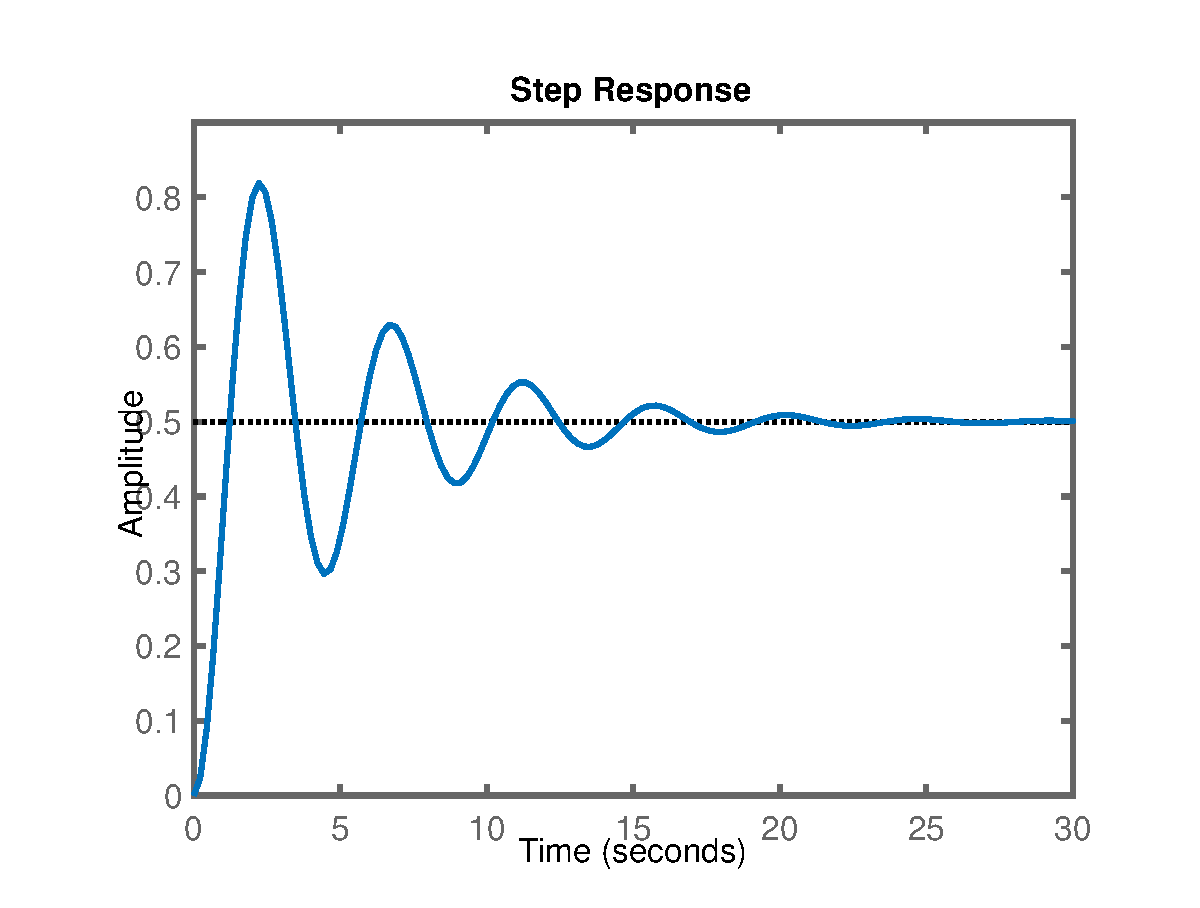
\includegraphics[width=0.8\linewidth]{Bilder/FreqCDesignStepResponse.eps}
	\caption{Step Response}
	\label{Fig_FreqCDStepResp}
\end{figure}
\begin{figure}[h!]
	\centering
	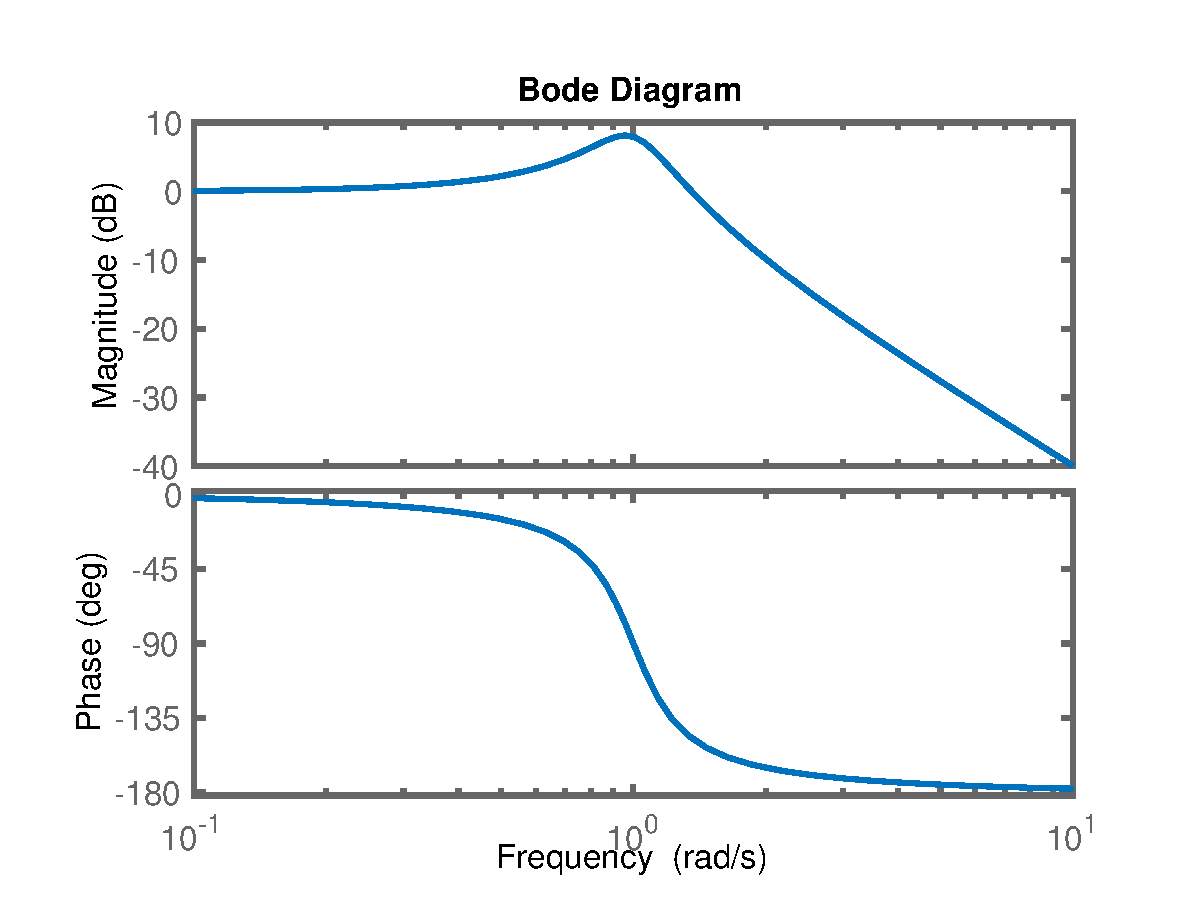
\includegraphics[width=0.8\linewidth]{Bilder/FreqCDesignFreqResp.eps}
	\caption{Frequency Response}
	\label{Fig_FreqCDFreqResp}
\end{figure}
\newpage
Generally, the close-loop time response is related to the open-loop frequency response for various parameters described earlier. For the case of a Type 0 system, the ss-error (closed-loop) is found using final value theorem:
\begin{equation}
	G_{CL}(s) = \frac{E(s)}{R(s)} = \frac{forward}{1 + loop} =  \frac{1}{1 + \frac{K}{s^2 + 0.4s + 1}} = \frac{s^2 + 0.4s + 1}{1 + K}
\end{equation}
In the forward path, there are no blocks between $R(s)$ and $E(s)$, in the loop there are blocks of $C(s) = K$ and $P(s)$.
The final value theorem is defined as follows:
\begin{equation}
	e_{ss} = \lim_{s\to 0} s E(s) \implies \lim_{s\to 0} s  \frac{s^2 + 0.4s + 1}{1 + K} R(s) = \lim_{s\to 0} s  \frac{s^2 + 0.4s + 1}{1 + K} \frac{1}{s}
\end{equation}
\begin{equation}
	e_{ss} = \frac{1}{1 + K}
\end{equation}
Looking at frequency response shown in figure \ref{Fig_FreqCDFreqResp}, the steady-state response in time-domain is due to an DC input (constant) at low frequency. Therefore, the magnitude response at lower frequencies will determine the ss-error from Bode plots. From figure \ref{Fig_FreqCDFreqResp}, at low frequencies the magnitude is $0 dB$ or $1$, therefore, there is a perfect tracking of the system w.r.t the input. At medium frequencies the magnitude amplifies indicating resonance and further at higher $\omega$, the magnitude attenuates. An attenuated magnitude at higher $\omega$ says that the system is not capable of tracking the input magnitude at higher input speeds $(\omega)$, therefore, this system does not have fast dynamics to take care of the faster inputs.

The speed of the system (rise time, peak time), that is the time required by the system to react to faster inputs is determined using the Bode plot magnitude response at higher frequencies as described earlier. As the input frequencies speed up in rad/s, the system as shown in figure \ref{Fig_FreqCDFreqResp} cannot keep up the magnitude. It essentially, attenuates the response as a result, therefore, it an input has to be given for the system, a faster input will not be followed by the system due to its slow dynamics. The rise time and peak times of this system will be larger. This is only the qualitative analysis so far, as we are not looking into exact numbers in terms of rise and settling times.

In terms of the overshoot in step-response, this behavior can be related at medium frequencies in Bode plot. It can be seen that the system overshoots (amplifies) at the region of medium frequencies. A step input fed into the system even only once will show such a behavior of medium frequency input just for one cycle. Therefore, this system as shown in figure \ref{Fig_FreqCDFreqResp}, shows tendencies of amplification in Bode plot, this amplification is related to the overshoot behavior in the time domain.

Summarizing the above results, the step response and frequency response of a system can be correlated for various parameters as below:
\begin{table}[h!]
	\centering
	\begin{tabular}{p{5cm} p{8cm}}
		\toprule
		\textbf{Low frequencies} & Relates the ss-error of step response \\
		\cmidrule{1-2}
		\textbf{Medium frequencies} & Relates the overshoot of step response \\
		\cmidrule{1-2}
		\textbf{High frequencies} & Relates the speed (rise time and settling time) of step response \\
		\bottomrule
	\end{tabular}
\end{table}

\begin{figure}[h!]
	\centering
	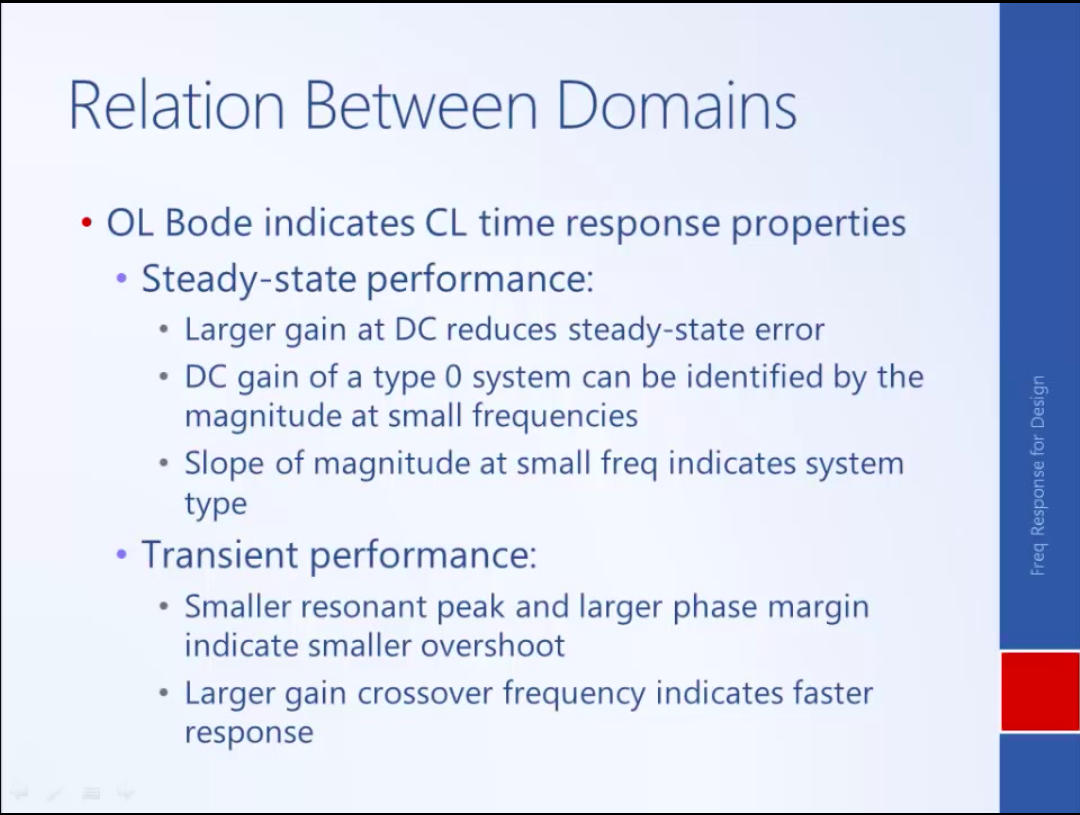
\includegraphics[width=\linewidth]{Bilder/FreqCDRelationships}
	\caption{Overview of time and frequency relationships}
\end{figure}

\section{Design with Frequency Response}

Once the relationships have been established between the time and the frequency response of the system, a controller is designed using the Bode plots. The controller is design to produce required effects in the time domain because ultimately the time response of a system is achieved in the real world. Such as its peak time (fastness), settling time and ss-error. The following steps can be laid down while designing a controller using frequency response:
\begin{enumerate}
	\item Analyse time response behavior and determine the parameters that needs to be improved
	\item Relate this parameters on the Bode plot
	\item Add a controller to change the shape of the frequency response so that it ultimately brings about the changes required in the time domain. The open-loop (OL) response of the system is considered for plotting Bode plots mainly because of two reasons:
	\begin{itemize}
		\item The OL response of a system determines its CL stability, as the magnitude and the phase shifts are evident in the OL, the CL then used the error generated by this OL response to implement a control.
		\item The OL Bode plot linearly adds the controller into the magnitude and phase plots as $G_{OL} = C(s)P(s)$, taking the log will add the products of the TF as seen in section \ref{Sec_BodePlotGain}. From the CL TF this linear addition of the controller is not possible as the TF will now become $G_{CL} = CP / 1 + CP$, therefore, the log will not add the controller linearly anymore.
	\end{itemize}
	\item The process of adding control gain and checking with the parameters is iterative mainly for two reasons:
	\begin{itemize}
		\item Magnitude and Phase plots are dependent of each other, changing one changes the response of another
		\item For non-canonical systems, the system parameters (settling time, overshoot etc.,) cannot be defined analytically, at this point the analysis will only be quantitative, therefore requires an iterative approach.
	\end{itemize}
\end{enumerate}

Consider the system shown in figure \ref{Fig_FreqCDStepResp} and \ref{Fig_FreqCDFreqResp}, if we decided that the systems has to be made much faster, reduce its overshoot and improve the ss-error. From the Bode plot figure \ref{Fig_FreqCDFreqResp}, the following changes has to be made:
\begin{itemize}
	\item Make system faster: Push the magnitude response (gain cross over frequency) in Bode plot to the right
	\item Reduce the overshoot: Particularly, the system phase margin has to be pushed upwards so that it has larger phase margin. By doing so, the constructive interference will be reduced at the summation point of the feedback inturn reducing the resonance of the system output. Also, the phase margin has to to be pushed upwards for the new gain margin that was achieved in earlier step so that the constructive interference is reduced at that point.
	\item Reduce the ss-error: ss-error is always reduced when the DC gain of the system is large enough (in P control a higher gain is given, I control does this by itself as it adds the pat errors). Essentially, the magnitude response in the Bode plot should be at low frequencies should be given a larger DC gain.
\end{itemize}

\subsection{Design with a lead compensator}

A lead compensator has a TF of a type:
\begin{equation} \label{Eq_TF_LC}
	C(s) = K \frac{s + z}{s + p}
\end{equation}
It has a simple zero and a pole and the zero is much smaller than a pole $(z << p)$. Therefore, the effect of zero will be dominating (at-least at higher frequencies when pole becomes more dominant). In essence, in a lead compensator, the effect of zero is tried to hit first in the system. In order to appreciate the effect of a lead compensator in the system, plot its Bode plot as given in figure \ref{Fig_FreqCDLeadBode}. The TF of lead compensator is initially written in Bode form as given below:
\begin{equation}
	C(s) = K \left(\frac{z}{p} \left( \frac{\frac{1}{z}s+1}{\frac{1}{p}s+1} \right) \right)
\end{equation}
For the purpose of generating a plot in Matlab random values of $1/z$ and $1/p$ are chosen in this case the values were chosen such that the break frequencies occur at $\omega = 2 rad/s$ for zero and $\omega = 3 rad/s$ for the pole (this was done by comparing the plants bode plot).
\begin{figure}[h!]
	\centering
	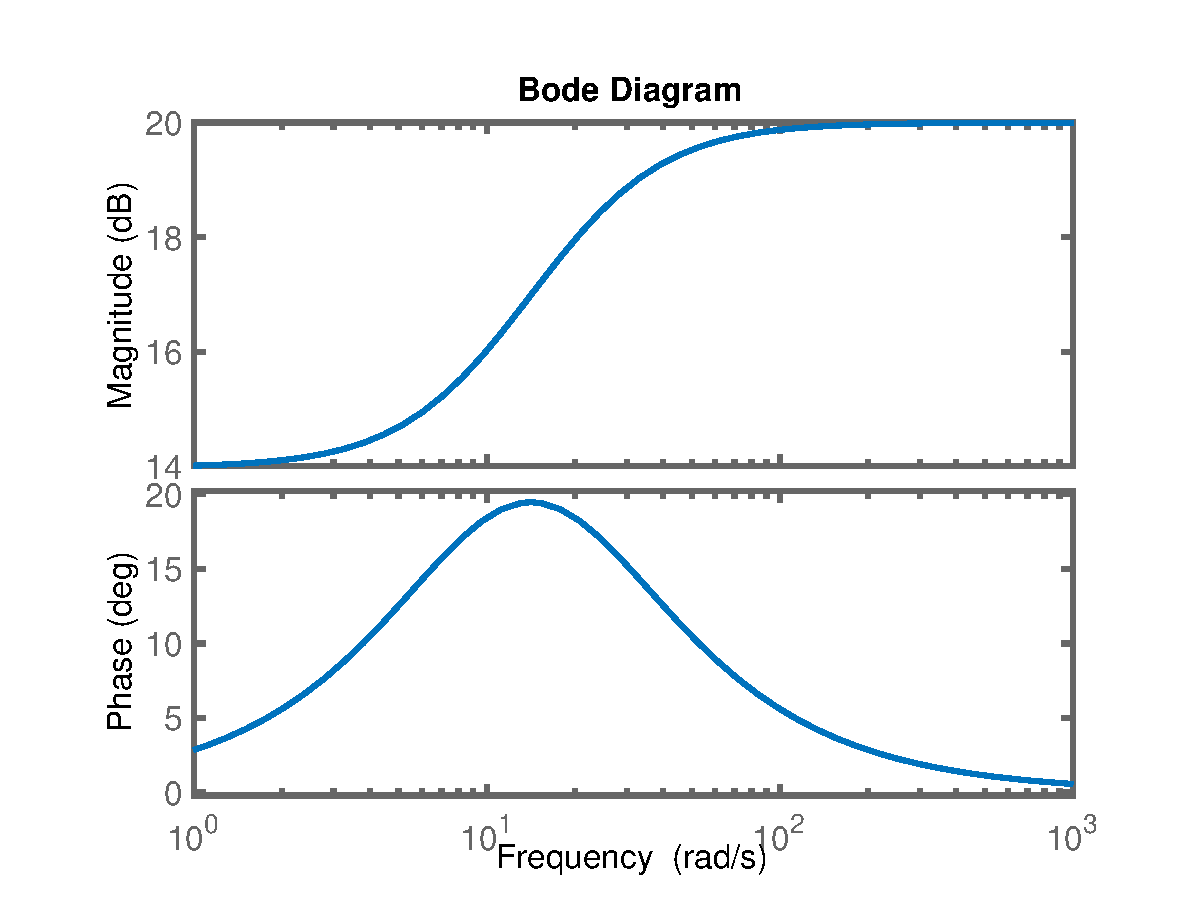
\includegraphics[width=0.8\linewidth]{Bilder/FreqCDLeadBode.eps}
	\caption{Bode plot of the lead compensator}
	\label{Fig_FreqCDLeadBode}
\end{figure}
\newpage
In order to understand the behavior of Lead compensator consider a straight-line approximation Bode plot as given in figure \ref{Fig_FreqCDLeadBodeSL}.
\begin{figure}[h!]
	\centering
	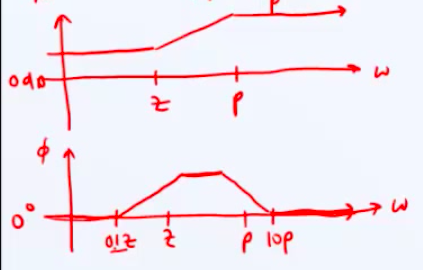
\includegraphics[width=0.8\linewidth]{Bilder/FreqCDLeadBodeSL}
	\caption{Bode plot of the lead compensator}
	\label{Fig_FreqCDLeadBodeSL}
\end{figure}

At low frequencies until the effect of zero hits the magnitude plot at $\omega = 1/z$, the magnitude is essentially a straight line with value $20 log K$. At cut-off frequency $\omega = 1/z$, the effect of zero hits in and the magnitude will increase with a slope of $20 dB / decade$, this should apparently go on increasing until the maximum $\omega$ but because of effect of pole hitting off at $\omega = 1/p$, the magnitude will now be influenced by the effect if pole with a decreasing slope $-20 dB / decade$. Since the effect if the both the slopes now interact and the overall effect will be to cancel the slope and make the magnitude a flat line after cut-off $\omega = 1/p$ as shown in figure \ref{Fig_FreqCDLeadBodeSL}.

In case of phase plots, at lower frequencies until the cut-off $\omega = 0.1z$ (a decade earlier when the slope starts), phase is zero. After which phase starts to increase such that the phase becomes constant of $90^{\circ}$ at $\omega = 10z$ (a decade later). Additionally, since the effect of pole starts to hit off at $\omega = 0.1p$, the phase becomes flat even earlier but not at $\omega = 10z$. However, after $\omega = 10z$, the effect of zero will run out as it should have become a constant line of $90^{\circ}$. The effect of pole to lag the phase continues until it reaches the cut-off $\omega = 10p$ so a lag in phase is seen further untill the point of $\omega = 10p$ after which the phase again becomes flat after the effect runs out at $\omega = 10p$.
\newpage
Plotting both the Bode plots of both the plant and controller, the following figure \ref{Fig_FreqCDSysBodeSL} can be produced.
\begin{figure}[h!]
	\centering
	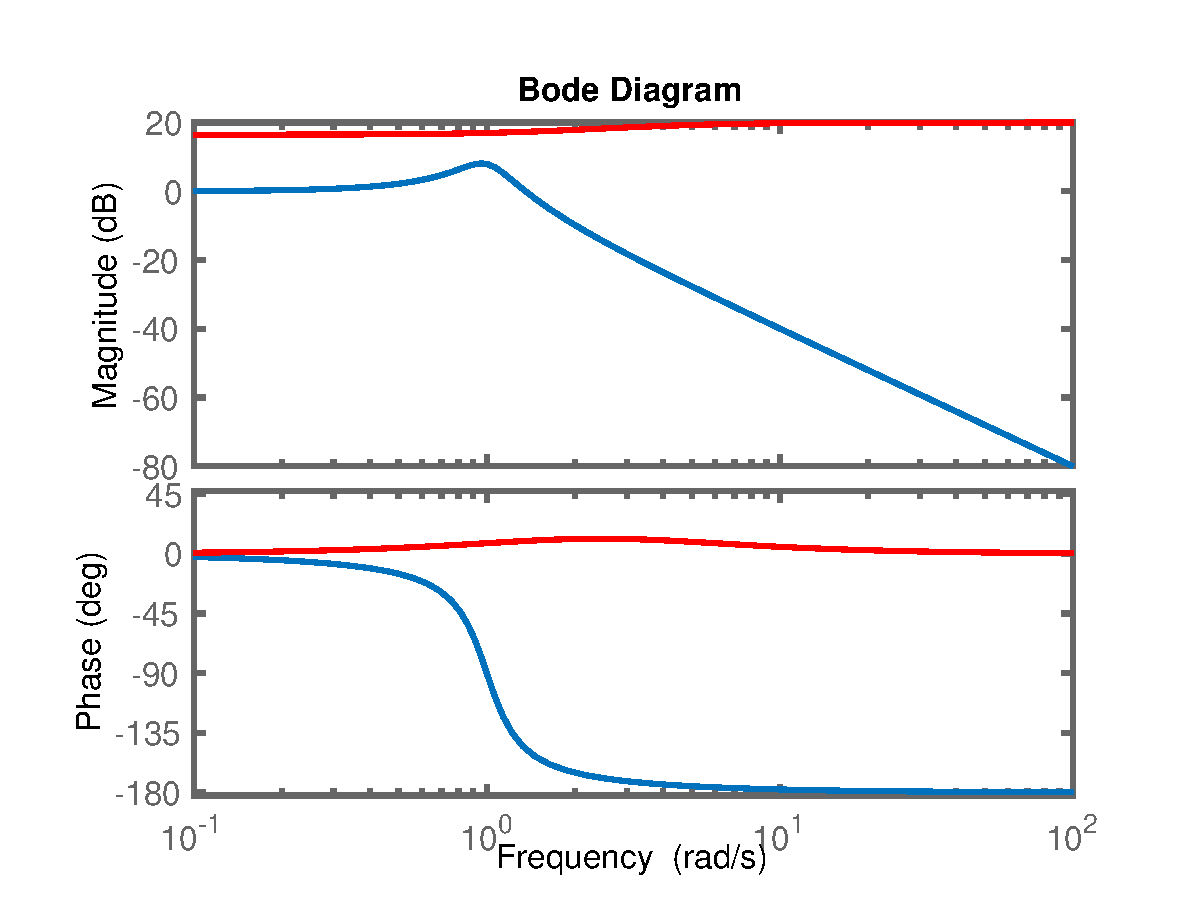
\includegraphics[width=0.8\linewidth]{Bilder/FreqCDSysBode.eps}
	\caption{Bode plot of the lead compensator and plant}
	\label{Fig_FreqCDSysBodeSL}
\end{figure}
\newpage
Further the effect of addition of a controller to the plant results in the following FrRe of the system in Bode plot (given by the yellow line) as shown in figure \ref{Fig_FreqCDTotBodeSL}.
\begin{figure}[h!]
	\centering
	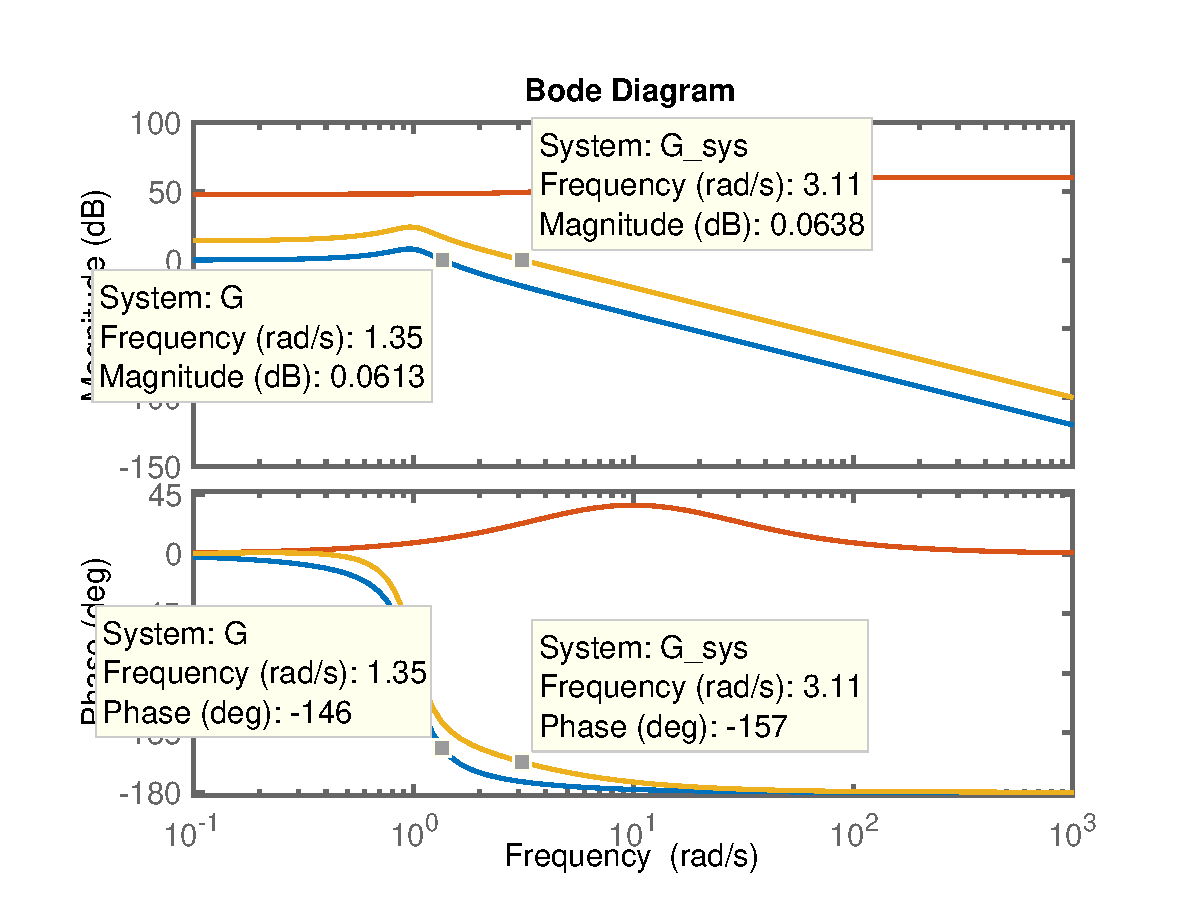
\includegraphics[width=0.8\linewidth]{Bilder/FreqCDTotBode.eps}
	\caption{Bode plot of plant with LC}
	\label{Fig_FreqCDTotBodeSL}
\end{figure}

It can be seen from figure \ref{Fig_FreqCDTotBodeSL}, (Yellow line) by using the LC quantitatively the objectives have been achieved by increasing the DC gain, pushing the gaim margin has been pushed to the right and the $P_m$ has been pushed upwards to reduce the constructive resonance which reduces the resonance of the system.

\subsection{Design with a PID controller}

\subsubsection{Design with a PD regulator}

In case a PD regulator is used in place of a LC, the behavior of the system can be determined using the Bode plot of $C(s)$. Writing the $C(s)$ in the Bode form, the following Bode plots can be generated:
\begin{equation}
	C(s) = K_D s + K_P = K (s + z) \implies K z \left( \frac{1}{z}s + 1 \right)
\end{equation}
where $z = K_P / K_D$. In comparison to a LC given by equation \eqref{Eq_TF_LC}, a PD control add only a zero. Consider the following Bode plot of a PD control as shwon in figure \ref{Fig_FreqCDPDBode}.
\begin{figure}[h!]
	\centering
	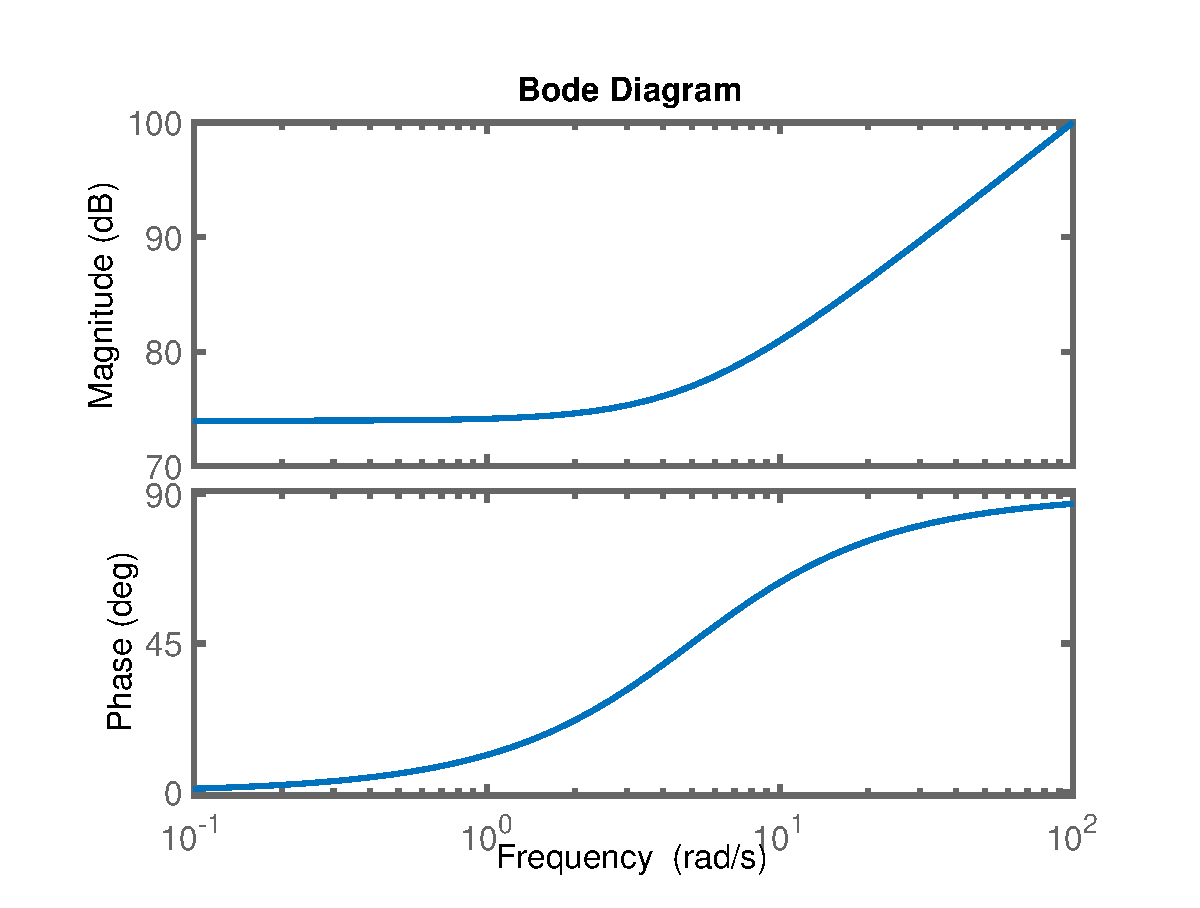
\includegraphics[width=0.8\linewidth]{Bilder/FreqCDPDBode.eps}
	\caption{Bode plot of plant with LC}
	\label{Fig_FreqCDPDBode}
\end{figure}

Since a PD control only adds a zero, after the cut-off $\omega$, the effect of the zero will kick-in and the MgRe increases with a positive slope of $20 dB/decade$. As there is no pole, this increase will continue till infinity $\omega$. It is evident from figure \ref{Fig_FreqCDPDBode}, at higher frequencies the MgRe amplifies to infinity and therefore using a PD control will induce the constructive resonance thereby increasing the resonance and making the system unstable. Also, it the input to the PD control is the noise (even though the error is attenuating), it will amplify the magnitude of noise and make the system unstable. In general, noise of of high frequency input to the system and a derivative type regulator always amplifies signals that are of high frequency.

\section{Comparison of Frequency based control design with Time based control design}

\subsection{Advantages of Frequency based control design}

\begin{enumerate}
	\item Provides rich source of information starting from a constant DC input to frequencies of any order
	\item ss-error information cannot be derived from time based design (pole placements), pole placements would determine the settling time, damping and other dynamic characteristics of the system but do not determine the ss-error. However, in Frequency based design, using Bode plots the MgRe of the system can be determined at any frequency.
	\item Settles the ambiguities from root locus (higher-order dynamics, effect of zeros): From root locus the effect of poles placed at far left in the Re plane do not show immediate effects in terms of time response, which is clearly visible in the Bode plots. Also, the effects of zeros in the MgRe and phase response is clearly seen in the Bode plots. So FrRe clarifies the effects of each terms (poles and zeros) of any system (lower or higher order systems).
	\item Good for experimental derivation (System Identification): Once the Bode plot of a system has been generated, the effects of each of the poles and zeros presents in the system can easily be identified which thereby effect the response properties such as gain cross-over and phase cross-over $\omega$, $G_m$, $P_m$ and others.
\end{enumerate}

\textbf{Advantages of Time response based control design}
\begin{itemize}
	\item The time response of a system directly gives the behavior of the systems response in the time domain, which is ultimately is required to be controlled. However, in most of the cases when the inputs are vary random with alternating frequencies, a qualitative comparison as perform in section \ref{Sec_RelationshipFrReTiRe} has to be done in order to relate the time-domain characteristics with FrRe and the design the controller.
\end{itemize}